% preamble
\documentclass{article}
\usepackage{fullpage}
\usepackage{fancyhdr}
\usepackage{graphicx}
\usepackage[headsep=1cm,total={6.5in, 8.5in}]{geometry}

% useful packages
\usepackage{amsmath,amssymb, amsthm}

% add your own packages here


% commands for header, fill in the appropriate values
\newcommand{\name}	{Manuel Rodriguez} % type name here
\newcommand{\settitle}	{Problem Set 1} %type set title here (ex. Problem Set 3, Midterm)
\newcommand{\latesub}	{No} % type yes/no indicating late submission

% a few helpful commands 
\newcommand{\RR}{\mathbb{R}} % typing \RR prints the Blackboard R used for Real Numbers
\newcommand{\NN}{\mathbb{N}} % typing \NN prints the Blackboard N used for Natural Numbers
\newcommand{\ZZ}{\mathbb{Z}} % typing \ZZ prints the Blackboard Z used for Integers

% construct your own commands here

\newcommand{\GCD}{\textrm{GCD}}


% commands for header, don't adjust
\begin{document}

\thispagestyle{empty}
\begin{center}\framebox{\vbox{ \vspace{2mm}
\hbox to 6.5in {\textbf{EE/CNS/CS~148~~~Topics in Computational Vision}\hfill \textbf{\today}} \vspace{4mm}
\hbox to 6.5in {\Large \hfill \settitle  \hfill} \vspace{2mm}
\hbox to 6.5in {\textbf{Name: } \name \hfill \textbf{Late Submission: } \latesub} \vspace{2mm}}
}\end{center} \vspace*{1mm}
\pagestyle{fancy}\lhead{Name: \name} \chead{\settitle} \rhead{\today}

\tableofcontents

% --------------------- Problem 1 ----------------------------
\newpage
\section{Generate the Dataset}
\subsection{A}
The data is going to be composed of points taken from two different, randomly-generated, Gaussian distributions. Without looking at the at plots, I would expect that the two classes are relatively different with the two having clearly different centers, but I would not expect the data to be linearly separable since it is unlikely that the centers are far apart and the uncertainties generated by both Gaussians are so small that there are no data points from the two distributions that are close together. Looking at the data, we can tell that there are two clear centers, but as expected, there is some overlapse in the middle of the graph.
\subsection{B}
For $dims=3$, I think the data would be more likely to be linearly separable since there are more degrees of freedom for the points to be distributed across and thus there is less of a chance that they will disperse along the same axis or have nearby centers.
\subsection{Controlling Randomness}

% Unfinished, missing one random aspect
\subsubsection{C}
An element of randomness that needs to be addressed for a perceptron is the set of points which are evaluated when determining error and updating weights. If these points are not chosen randomly, there would be a bias toward fitting for the first points in the model which could be fatal if the points are ordered, for example, by simple ascending order. Another element of randomness to consider is the initial values of all the weights, obviously they cannot be zero because then you face vanishing gradients, but also they must not be biased toward any particular target function, so a popular choice if initializing the weights to small, normally distributed values. Another element of randomness that could be addressed is the sampling of your data points. If your data points aren't actually sampled from the distribution you are trying to replicate (because of some bias in your system of sampling) the accuracy of your model on the test point will be poor and inaccurate.
\subsubsection{D}
Done :D

% --------------------- Problem 2 ----------------------------
\newpage
\section{Compute Backprop + Code}
\subsection{A, B, C}
\includegraphics*[width=16cm]{../figs/Q2_a_b_c.pdf}
\subsection{D}
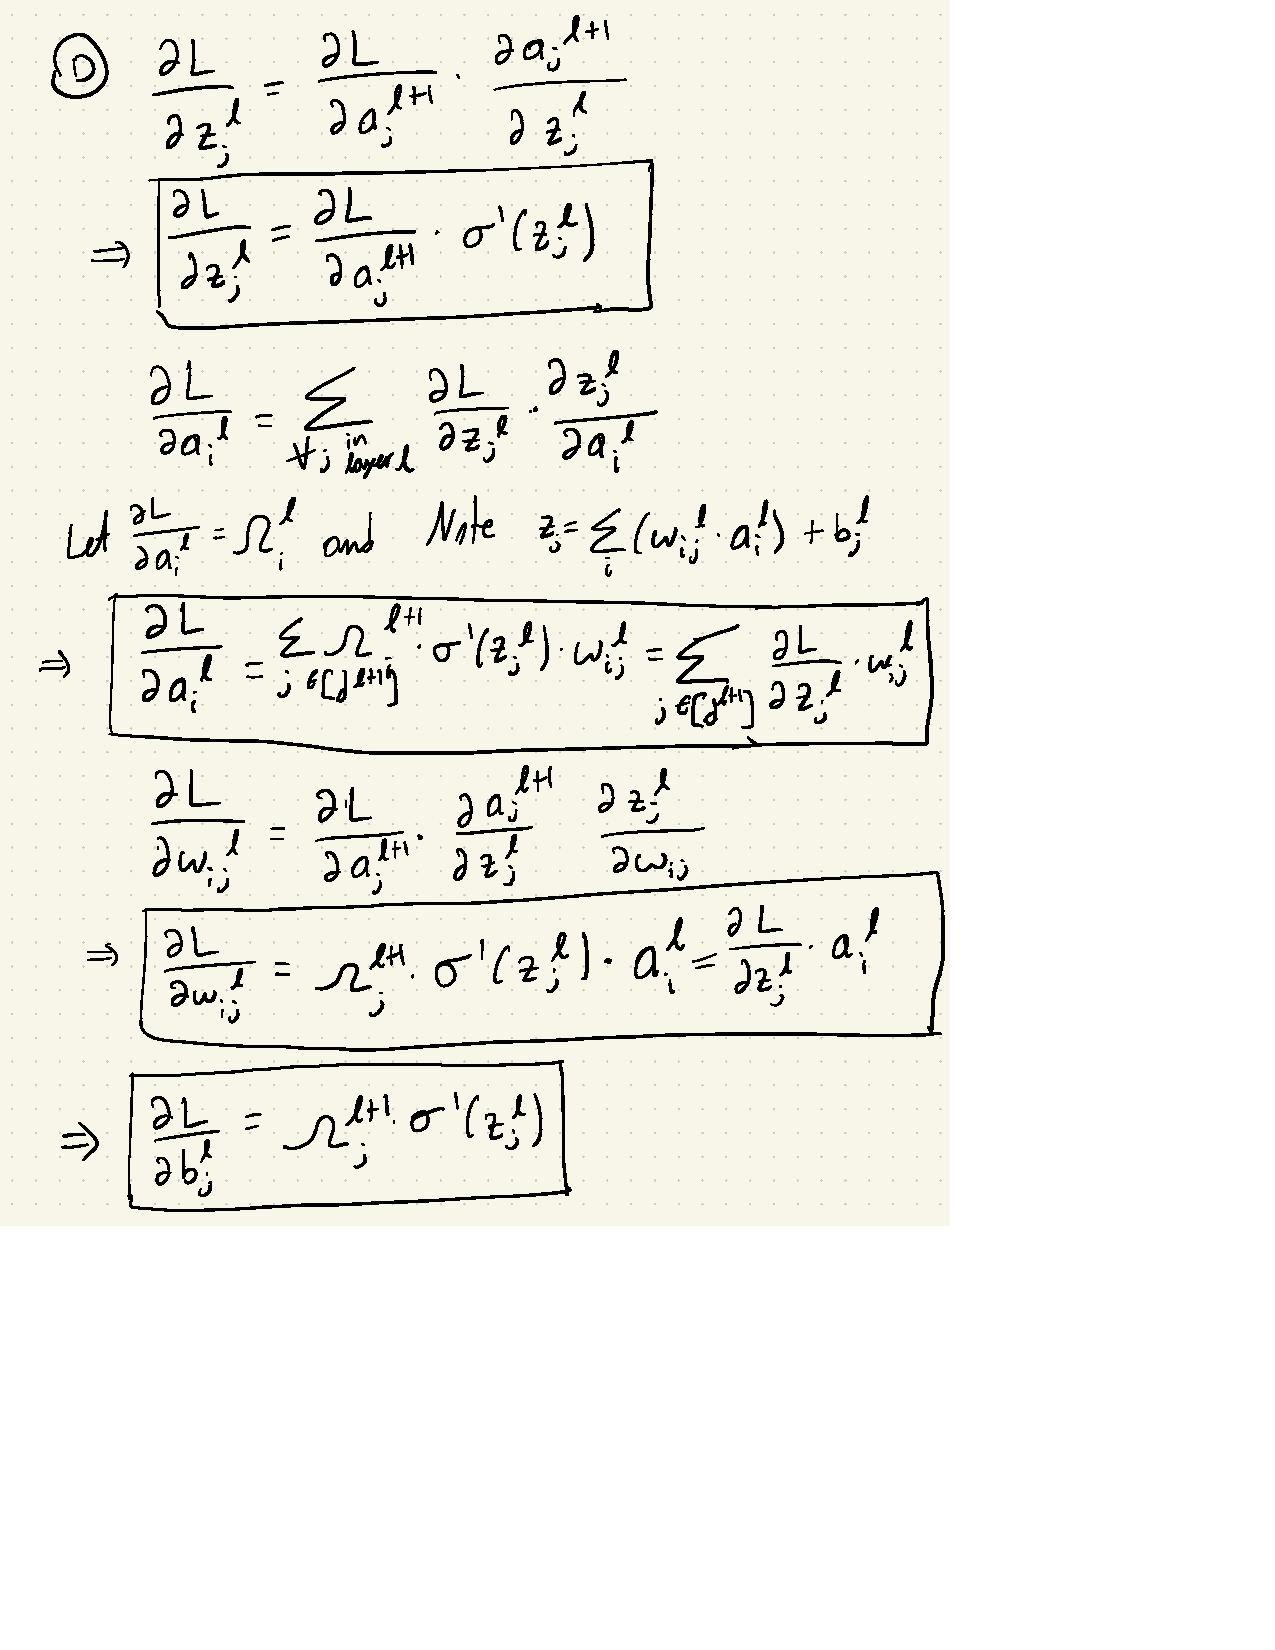
\includegraphics[width=13cm]{../figs/Q2_d.pdf}
\subsection{E}
We choose to formulate backpropagation in this way because it lends itself to a lot of repeated subproblems. The derivatives for later layers appear in the calculations for previous layers and this makes it so that if we store our derivatives for activations and signals for later layers, then we can calculate in linear time each single activation of the current layer. In fact, each derivative is only dependent on the layer immediately after it.
\subsection{F}
\graphicspath{{../figs/}} 
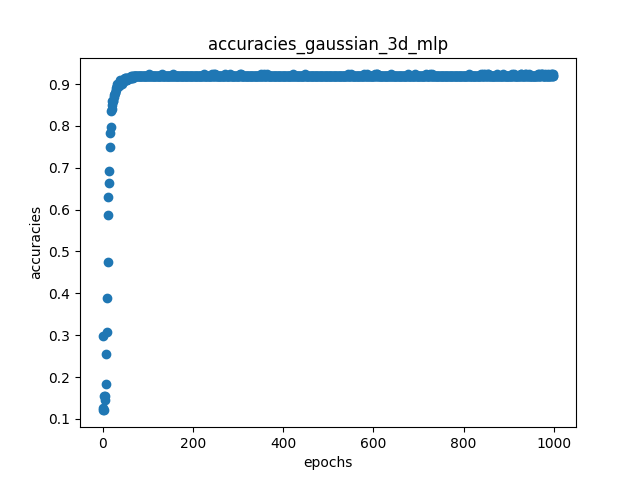
\includegraphics{accuracies_gaussian_3d_mlp.png} \\
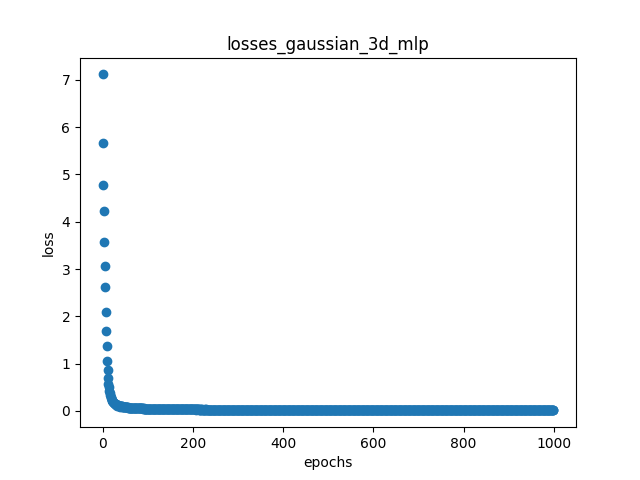
\includegraphics{losses_gaussian_3d_mlp.png}

% --------------------- Problem 3 ----------------------------
\newpage
\section{Compare Dataset Distributions}
Here are the accuracies and losses for the concentric circles and iris datasets. \\
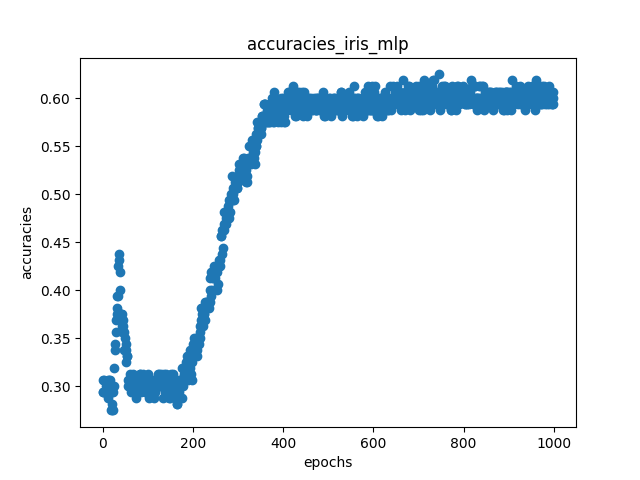
\includegraphics[width=8cm]{accuracies_iris_mlp}
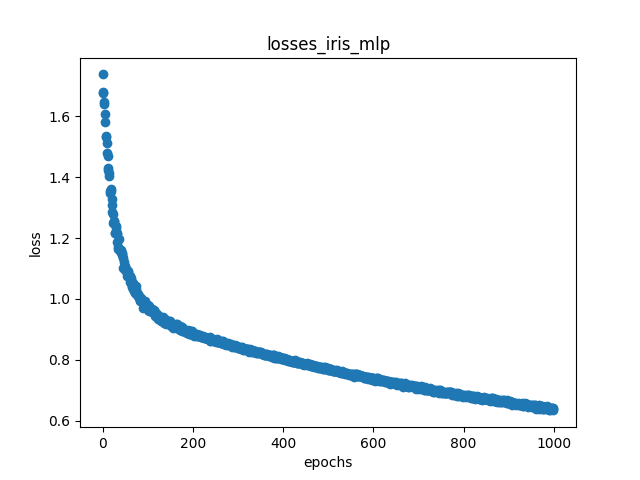
\includegraphics[width=8cm]{losses_iris_mlp}
\\
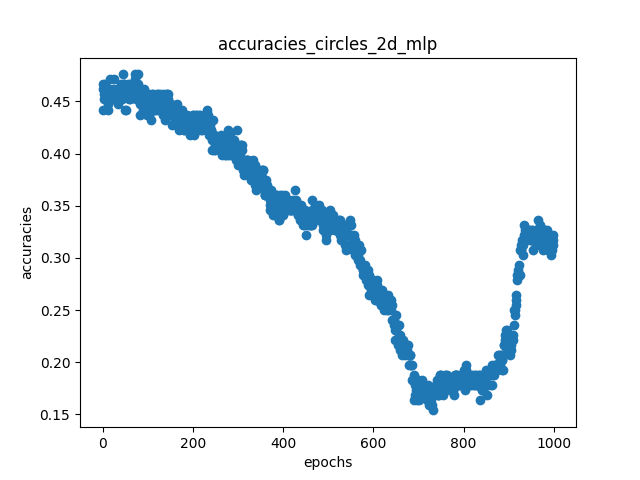
\includegraphics[width=8cm]{accuracies_circles_2d_mlp}
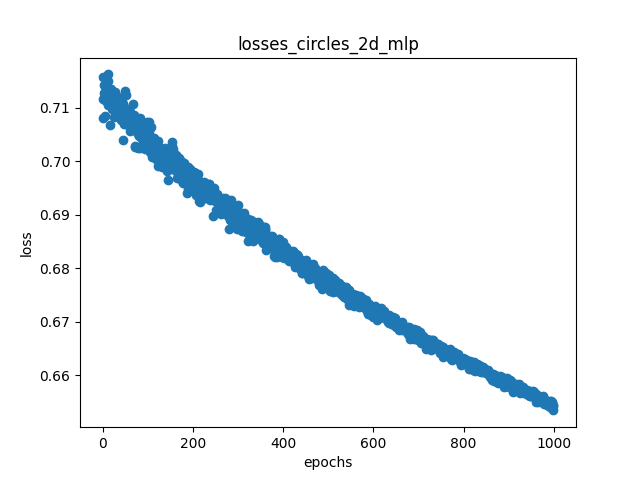
\includegraphics[width=8cm]{losses_circles_2d_mlp}
\subsection{A}
An MLP with one hidden layer is incapable of solving this kind of classification problem because each MLP layer can only learn lines. To do this classification, the MLP would need another layer that can serve as an AND that can combine all these lines together to make a bounding box around the spherical data in the middle which is not linearly separable.
\subsection{B}
Because the Iris dataset is a multiclass problem, it is unlikely that the data will be linearly separable and will need a more complicated model similarly to the kCircles dataset so that it can identify which sections of the feature space correspond to which classes. 

% --------------------- Problem 4 ----------------------------
\newpage
\section{Plots + Hyperparameter Sweeps and Effects}
\subsection{A}
Done.
\subsection{B Learning Rate}
\subsubsection{i}
Below we can see that for the Gaussian, the best learning rate was around $10^{-3}$, for the kCircles it was around $10^{-1}$, and for the kIris it was around $10^{-2}$. The kCircles is able to get close to zero test error for three values of the learning rate which suggests that there is a clear 'sweet spot' in terms of finding the minimum of the loss function. \\
\includegraphics*[width=18cm]{learning_rate}
\subsubsection{ii}
The loss explodes for high learning rates because the weights are just jumping around the Loss function at different points, completely overshooting the local minimum of the function.
\subsubsection{iii}
When the learning rate is low, it takes too long to learn anything and the weights of the network barely change even if the loss is terrible and gradient is large.
\subsection{C Epochs}
\subsubsection{i}
Below we see that $10^4$ epochs gives a clear best performance for the Gaussian distribution but for the Circles and Iris datasets $10^2$ and $10^3$ respectively give very low test error and with the Iris dataset the test error actually increases at $10^4$ epochs. This means that Iris is asked the simplest task in some way such that training for too long leads to overfitting whereas on the other extreme, the Gaussian data needs the most amount of time to learn and benefits from more epochs.\\
\includegraphics*[width=16cm]{epochs}
\subsubsection{ii}
\begin{align*}
Gaussian &| Test: Never - Train: Never \\
Circles &| Test: 10^2 - Train: 10^2 \\
Iris &| Test: 10^3 - Train: 10^3
\end{align*}
\subsubsection{iii}
In the Gaussian dataset there is no convergence because the loss has not yet gotten close to a minimum and seems to be approaching lower and lower loss values but has not yet reached a plateau. Over more epochs, it is likely that the Gaussian dataset will converge.\\
\includegraphics*[width=16cm]{epoch_gradients}
\subsubsection{iv}
In the Iris dataset we see clear overfitting happening when we go to $10^4$ epochs since the loss shoots up as compared to the local minimum that was seen at $10^3$ epochs.
\subsubsection{v}
Three common techniques to prevent overfitting are to reduce model complexity, use regularization, and using dropout. They each can be optimal choices and through testing and Hyperparameter sweeps one can determine which give the best results for a given problem.
\subsection{Batch Size}
\subsubsection{i}
The best batch sizes for the Gaussian data was around 5, for the Circles data was around 1-2, and for the Iris dataset it was around 10.\\
\includegraphics*[width=16cm]{batch_size}
\subsubsection{ii}
It can be noted that there is no general rule to decrease the loss according to batch size, however, in general, a greater batch size seems to make the test error follow the training error more tightly.
\subsubsection{iii}
A smaller batch size will make your experiment run quicker since runtime is directly proportional to the number of elements in a batch. For larger batches, it will take longer to calculate gradients and finish each epoch.

\subsection{Training Samples}
\subsubsection{i}
We note that for the Gaussian dataset, we observe a minimum in the test error at around $100$ sample points whereas for the more complicated task of the Circles dataset, we get a minimum at around $1000$ sample points.\\
\includegraphics*[width=16cm]{training_size_differences}
\subsubsection{ii}
Unbalanced dataset distributions are a tradeoff between training power and reliability of results. If there is a fixed amount of data, using a greater training split is desirable because it will better train the model, potentially at the cost of overfitting, but will give you less reliable results for the estimate of the true accuracy/error.
\subsubsection{iii}
Error changes across the different datasets because the complexity of classifying each task determines the amount of training data that is suitable for each network. According to the graphs, the Circles dataset has a more complex task because it requires more training data to get the same low error that the Gaussian dataset gets for smaller training data.

\subsection{Layer Depth vs Width}
\subsubsection{i}
For the Gaussian dataset, both the thin and wide network perform about the same, but for the Iris and Circles datasets, the wide network performs significantly better. This might be due to the idea that a thin layer in a network acts as a compression of information while a wide layer acts as an interpretation of the dataset. So when the complicated tasks of Iris and Circles get passed through the thin network, not much useful information is passed through any one layer leading to loss of information which makes it difficult for the network to learn. On the other hand, in the wide network, the model can break these tasks down into subproblems which can then each be solved building on each other, such as creating a bounding box from many perceptrons. \\
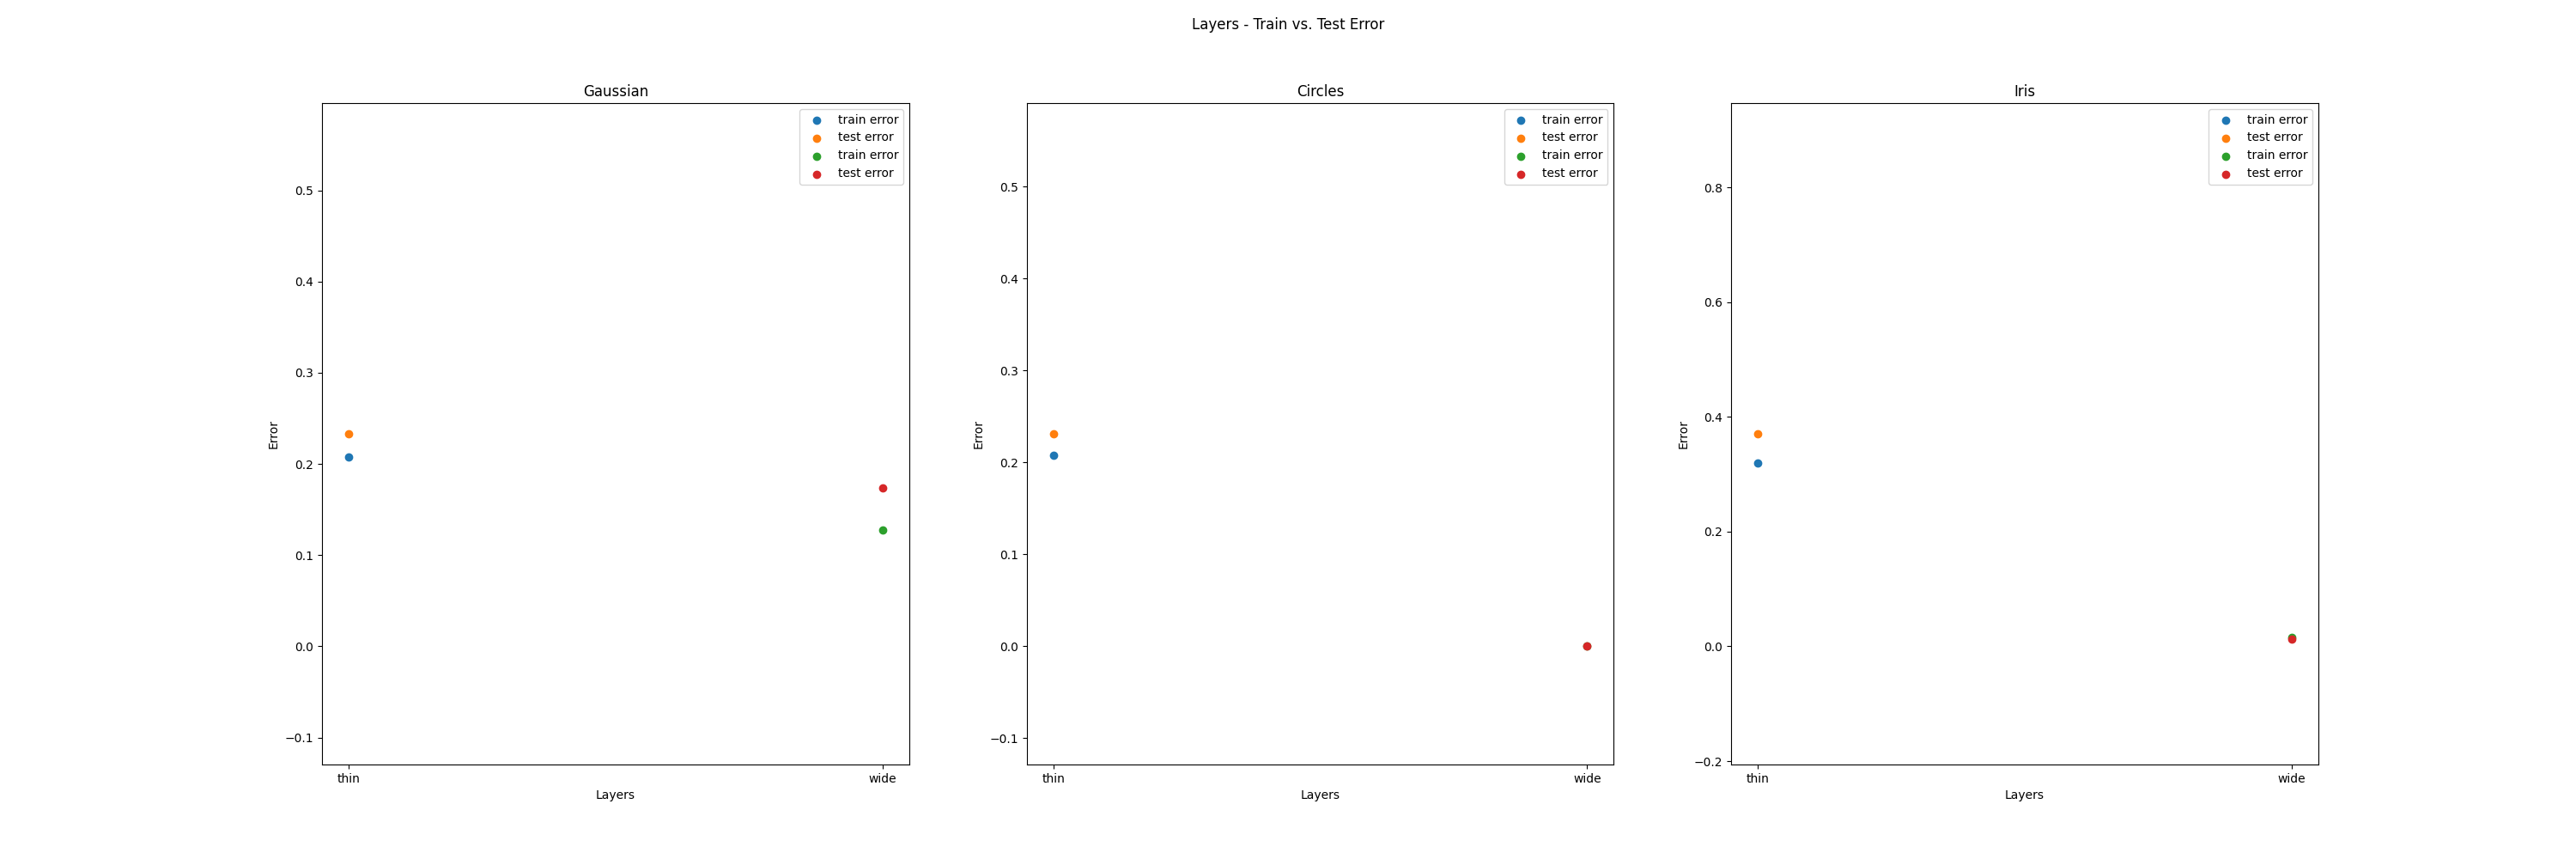
\includegraphics[width=16cm]{layer_sizes}

% --------------------- Problem 5 ----------------------------
\newpage
\section{Intuition for Activation and Loss Functions}
\includegraphics*[width=16cm]{activation_func}
\subsection{A}
Changing the activation function to ReLU, we get almost a $50\%$ drop in our error. This is likely due to the fact that ReLU gets rid of the vanishing gradients problem that is prominent to the sigmoid activation function due to its tangents to $y = 1$ and $y = -1$ when $\|x\|$ is large. This provides diminishing returns in our backpropagation for values that should really be very influential because they are unexpected.
\subsection{B}
Replacing the activation function to tanH, we get another almost $50\%$ drop in our error. This could be due to ReLU skipping around too much to find the local minimum. tanH is slower than ReLU to converge and thus may have stumbled onto a local minimum faster than ReLU, because ReLU's steps were too large.
\includegraphics*[width=16cm]{loss_func}
\subsection{C}

Changing the loss function to Hinge Loss and Mean Squared Error greatly decreased the error. Though these numbers look smaller, they are not necessarily better since all of these loss functions' error values only make sense in relation to themselves and comparison to itself. However, it is possible that changing the loss function can be very beneficial if that new loss function is more suitable to calculating the error of your measurements. For example, if you are trying to train a linear classifier on a set of linearly separable points, then using something like negative log likelihood will likely not give you as good-looking of a line as just using MSE.

\end{document}